\documentclass[10pt,final,a4paper,oneside,onecolumn]{article}

%%==========================================================================
%% Packages
%%==========================================================================
\usepackage[a4paper,left=3.5cm,right=3.5cm,top=3cm,bottom=3cm]{geometry} %% change page layout; remove for IEEE paper format
\usepackage[T1]{fontenc}                        %% output font encoding for international characters (e.g., accented)
\usepackage[cmex10]{amsmath}                    %% math typesetting; consider using the [cmex10] option
\usepackage{amssymb}                            %% special (symbol) fonts for math typesetting
\usepackage{amsthm}                             %% theorem styles
\usepackage{dsfont}                             %% double stroke roman fonts: the real numbers R: $\mathds{R}$
\usepackage{mathrsfs}                           %% formal script fonts: the Laplace transform L: $\mathscr{L}$
\usepackage[pdftex]{graphicx}                   %% graphics control; use dvips for TeXify; use pdftex for PDFTeXify
\usepackage{array}                              %% array functionality (array, tabular)
\usepackage{upgreek}                            %% upright Greek letters; add the prefix 'up', e.g. \upphi
\usepackage{stfloats}                           %% improved handling of floats
\usepackage{multirow}                           %% cells spanning multiple rows in tables
%\usepackage{subfigure}                         %% subfigures and corresponding captions (for use with IEEEconf.cls)
\usepackage{subfig}                             %% subfigures (IEEEtran.cls: set caption=false)
\usepackage{fancyhdr}                           %% page headers and footers
\usepackage[official,left]{eurosym}             %% the euro symbol; command: \euro
\usepackage{appendix}                           %% appendix layout
\usepackage{xspace}                             %% add space after macro depending on context
\usepackage{verbatim}                           %% provides the comment environment
\usepackage[dutch,USenglish]{babel}             %% language support
\usepackage{wrapfig}                            %% wrapping text around figures
\usepackage{longtable}                          %% tables spanning multiple pages
\usepackage{pgfplots}                           %% support for TikZ figures (Matlab/Python)
\pgfplotsset{compat=1.14}						%% Run in backwards compatibility mode
\usepackage[breaklinks=true,hidelinks,          %% implement hyperlinks (dvips yields minor problems with breaklinks;
bookmarksnumbered=true]{hyperref}   %% IEEEtran: set bookmarks=false)
%\usepackage[hyphenbreaks]{breakurl}            %% allow line breaks in URLs (don't use with PDFTeX)
\usepackage[final]{pdfpages}                    %% Include other pdfs
\usepackage[capitalize]{cleveref}				%% Referensing to figures, equations, etc.
\usepackage{units}								%% Appropriate behavior of units
\usepackage[utf8]{inputenc}   				 	%% utf8 support (required for biblatex)
\usepackage{csquotes}							%% Quoted texts are typeset according to rules of main language
\usepackage[style=ieee,doi=false,isbn=false,url=false,date=year,minbibnames=15,maxbibnames=15,backend=biber]{biblatex}
%\renewcommand*{\bibfont}{\footnotesize}		%% Use this for papers
\setlength{\biblabelsep}{\labelsep}
\bibliography{../../bib}

%%==========================================================================
%% Define reference stuff
%%==========================================================================
\crefname{figure}{Figure}{Figures}
\crefname{equation}{}{}

%%==========================================================================
%% Define header/title stuff
%%==========================================================================
\newcommand{\progressreportnumber}{34}
\renewcommand{\author}{Erwin de Gelder}
\renewcommand{\date}{October 8, 2020}
\renewcommand{\title}{Performance assessment of automated vehicles using real-world driving scenarios}

%%==========================================================================
%% Fancy headers and footers
%%==========================================================================
\pagestyle{fancy}                                       %% set page style
\fancyhf{}                                              %% clear all header & footer fields
\fancyhead[L]{Progress report \progressreportnumber}    %% define headers (LE: left field/even pages, etc.)
\fancyhead[R]{\author, \date}                           %% similar
\fancyfoot[C]{\thepage}                                 %% define footer

\begin{document}
	
\begin{center}
	\begin{tabular}{c}
		\title \\ \\
		\textbf{\huge Progress report \progressreportnumber} \\ \\
		\author \\ 
		\date
	\end{tabular}
\end{center}

\section{Previous meeting minutes}

\begin{itemize}
	\item We discussed the planning for my fourth year in more detail. There were no objections regarding the planning of the publications. For the final dissertation, I got the tip to bundle the articles I have written while only correcting mistakes and reformatting things like figures. Fixing the notation to be consistent across the different articles is not necessary.
	
	\item Regarding the paper ``Towards an Ontology for the Scenario Definition for the Assessment of Automated Vehicles: An Object-Oriented Framework'', it was suggested to submit it to \emph{Transactions of Intelligent Vehicles}. As a backup, \emph{IEEE Access} and \emph{IET Intelligent Transport Systems} could be considered.
\end{itemize}

\section{Summary of work}

\begin{itemize}
	\item I received and processed feedback from Jan-Pieter, Hala, Olaf, Steven Kraines, and Jeroen Ploeg for the paper ``Towards an Ontology for the Scenario Definition for the Assessment of Automated Vehicles: An Object-Oriented Framework''. I recently received feedback from Arash, but his feedback is contradicting the feedback from the other authors. I planned a call with him to see if we can easily address his concerns without changing too much. The latest version is attached to this report. My goal is to submit the article to Transactions of Intelligent Vehicles this month.
	
	\item I worked on the code implementation of the object-oriented framework. The code is publicly available\footnote{\url{https://github.com/ErwindeGelder/ScenarioDomainModel}}. Currently, there are two tutorials explaining how the code works. I want to add two more tutorials; one on how to create a scenario from raw data and one on how to use the code to manage a scenario database. I hope that these two tutorials demonstrate how the proposed framework complements existing implementations such as OpenSCENARIO. I want to have this finished before submitting the manuscript.
	
	\item I continued my work regarding the risk quantification. To illustrate the method, a case study is done. In this case study, I want to estimate the probability of a collision in certain types of scenarios. The problem I am currently facing is that the probabilities of collisions are extremely low, e.g., as low as $10^{-10}$. This is mainly caused by the somewhat idealized model of the driver that is used. Although the method is still working, I think it would be better to have more realistic driver models in order to convey the use of the method. I looked at different driver models \autocite{hamdar2008modeling, hamdar2015behavioral}, but I have not finished this yet.
	
	\item I already wrote part of the method for the risk quantification. This is attached to this report (starting at page 25).
\end{itemize}

\section{Future plans}

%In \cref{fig:planning}, the updated planning is shown. There are a few changes compared to the planning shown in the previous progress report:
%\begin{itemize}
%	\item 
%\end{itemize}
%
%\begin{figure}[t]
%	\centering
%	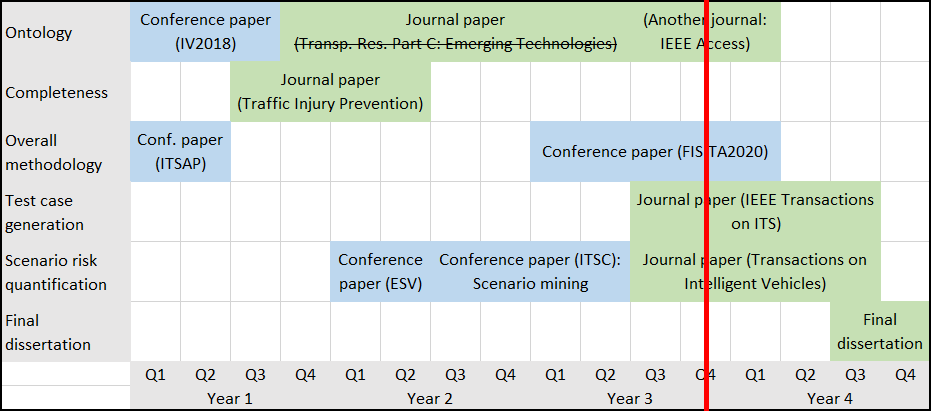
\includegraphics[width=\linewidth]{planning.png}
%	\caption{Proposed planning at the time of this report. The red line indicated the time when writing this report.}
%	\label{fig:planning}
%\end{figure}

\begin{itemize}
	\item Submit the paper ``Towards an Ontology for the Scenario Definition for the Assessment of Automated Vehicles: An Object-Oriented Framework'' to \emph{Transactions on Intelligent Vehicles}. 
	\item Finish the case study for the risk quantification.
\end{itemize}

\section{Questions}

\begin{itemize}
	\item The paper ``Towards an Ontology for the Scenario Definition for the Assessment of Automated Vehicles: An Object-Oriented Framework'' is now 15 pages long (including references and appendix). IEEE suggests that `regular papers' should have a length of 10 pages (for each extra page, an overlength charge needs to be paid). Could the paper length be an issue for a reviewer? If so, I might need to shorten the paper at least one to two pages, e.g., by leaving out some references (now there are 74 references).
	
	\item This month, I started by fourth year. Could we plan a yearly progress meeting? Perhaps during the next regular progress meeting?
\end{itemize}


\printbibliography

\clearpage
\includepdf[pages=-,pagecommand={},width=\paperwidth]{../../"20180629 Journal paper ontology"/framework_scenarios.pdf}
\includepdf[pages=-,pagecommand={},width=\paperwidth]{../../"20191113 Journal Scenario Risk"/scenario_risk.pdf}

\end{document}